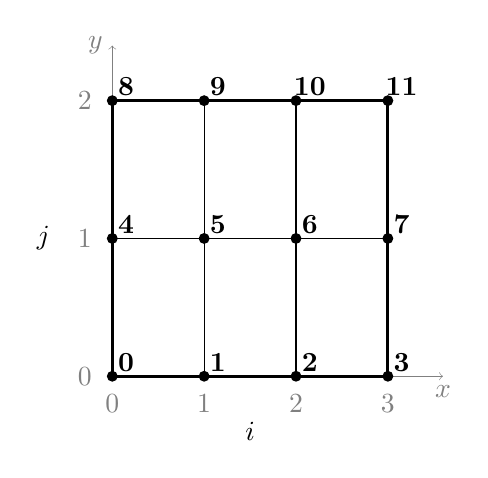
\begin{tikzpicture}[scale=3.5]
  \draw[->,gray,very thin] (0.0,0.0) -- (1.2,0.0) node[below] {$x$};
  \draw[->,gray,very thin] (0.0,0.0) -- (0.0,1.2) node[left] {$y$};
  \draw[line width=1.0pt] (0.0,0.0) -- (0.0,1.0) -- (1.0,1.0) -- (1.0,0.0) -- cycle;
  \pgfmathsetmacro\third{1.0/3.0}
  \pgfmathsetmacro\half{1.0/2.0}
  \node[gray] at (0.0,-0.1) {$0$};
  \node[gray] at (\third,-0.1) {$1$};
  \node at (\half,-0.2) {$i$};
  \node[gray] at (2*\third,-0.1) {$2$};
  \node[gray] at (1.0,-0.1) {$3$};
  \node[gray] at (-0.1,0.0) {$0$};
  \node[gray] at (-0.1,0.5) {$1$};
  \node at (-0.25,0.5) {$j$};
  \node[gray] at (-0.1,1.0) {$2$};
  \draw[xstep=\third,ystep=\half,black,thin] (0.0,0.0) grid (1.0,1.0);
  \pgfmathsetmacro\dd{0.05}
  \foreach \y in {0,1,2}
    \foreach \x in {0,1,2,3} {
      \pgfmathsetmacro\k{4*\y+\x}
      \draw (\x*\third+\dd,\y*\half+\dd) node{$\mathbf{\pgfmathprintnumber[fixed]{\k}}$};
      \filldraw (\x * \third,\y * \half) circle (0.5pt);
    }
\end{tikzpicture}

